%%%%%%%%%%%%%%%%%%%%%%%%%%%%%%%%%%%%%%%%%%%%%%%%%%%%%%%%%%%%%%%%%%%%%%%%
% Slide options
%%%%%%%%%%%%%%%%%%%%%%%%%%%%%%%%%%%%%%%%%%%%%%%%%%%%%%%%%%%%%%%%%%%%%%%%

% Option 1: Slides with solutions

\documentclass[slidestop,compress,mathserif]{beamer}
\usepackage{booktabs}
\newcommand{\soln}[1]{\textit{#1}}
\newcommand{\solnGr}[1]{#1}

% Option 2: Handouts without solutions

%\documentclass[11pt,containsverbatim,handout]{beamer}
%\usepackage{pgfpages}
%\pgfpagesuselayout{4 on 1}[letterpaper,landscape,border shrink=5mm]
%\newcommand{\soln}[1]{ }
%\newcommand{\solnGr}{ }

%%%%%%%%%%%%%%%%%%%%%%%%%%%%%%%%%%%%%%%%%%%%%%%%%%%%%%%%%%%%%%%%%%%%%%%%
% Style
%%%%%%%%%%%%%%%%%%%%%%%%%%%%%%%%%%%%%%%%%%%%%%%%%%%%%%%%%%%%%%%%%%%%%%%%
%%%%%%%%%%%%%%%%%%%%%%%%%%%%%%%%%%%%%%%%%%%%%%%%%%%%%%%%%%%%%%%%%%%%%%%%
% MA213/214 shared slide style
%
% "Calm & Cool" palette + content-type callout boxes.
% Overhauled (2026) from the original OpenIntro/metropolis style:
%   - all OpenIntro visual branding removed (logo, grid, colors)
%   - a low-key cool palette (see colors below)
%   - tcolorbox callout boxes so students recognize content types
% See common/README.md for the command cheat-sheet.
%%%%%%%%%%%%%%%%%%%%%%%%%%%%%%%%%%%%%%%%%%%%%%%%%%%%%%%%%%%%%%%%%%%%%%%%

\usetheme{metropolis}

%%%%%%%%%%%%%%%%
% Packages
%%%%%%%%%%%%%%%%

\usepackage{geometry}
\usepackage{graphicx}
\usepackage{amssymb}
\usepackage{epstopdf}
\usepackage{amsmath}  	% this permits text in eqnarray among other benefits
\usepackage{url}		% produces hyperlinks
\usepackage{hyperref}	% allows for color usage in tables
\usepackage[english]{babel}
\usepackage[latin1]{inputenc}
\usepackage{colortbl}	% allows for color usage in tables
\usepackage{multirow}	% allows for rows that span multiple rows in tables
\usepackage{color}		% this package has a variety of color options
\usepackage{pgf}
\usepackage{calc}
\usepackage{ulem}
\usepackage{multicol}
\usepackage{textcomp}
\usepackage{txfonts}
\usepackage{listings}
\usepackage{tikz}
\usepackage{array}
\usepackage{wasysym}
\usepackage{fancyvrb}
\usepackage{etoolbox}             % \ifstrempty for optional box subtitles
\usepackage[most]{tcolorbox}      % content-type callout boxes
\tcbuselibrary{listings}          % R-code block (\begin{rblock})
\usepackage{fontawesome5}         % box icons

%%%%%%%%%%%%%%%%
% Remove navigation symbols
%%%%%%%%%%%%%%%%

\setbeamertemplate{navigation symbols}{}

%%%%%%%%%%%%%%%%
% "Calm & Cool" palette
%%%%%%%%%%%%%%%%

% chrome / structure / body
\definecolor{ccSlate}{HTML}{2E3742}   % frametitle bar, structure, section pages (deep neutral slate)
\definecolor{ccInk}{HTML}{2B2B2B}     % body text
\definecolor{ccWash}{HTML}{FCF8F1}    % gentle warm title-slide background wash (complements the cool blues)

% example (blue)
\definecolor{ccBlue}{HTML}{2F6690}
\definecolor{ccBlueBg}{HTML}{EAF1F7}
% interactive activity / discussion (green)
\definecolor{ccGreen}{HTML}{4E8A6B}
\definecolor{ccGreenBg}{HTML}{E9F3EC}
% solution (purple)
\definecolor{ccPurple}{HTML}{6F5499}
\definecolor{ccPurpleBg}{HTML}{EFEAF6}
% worksheet / focused work (terracotta)
\definecolor{ccTerra}{HTML}{C2693E}
\definecolor{ccTerraBg}{HTML}{FAEDE4}
% formula / definition (neutral slate)
\definecolor{ccGray}{HTML}{5C6B7A}
\definecolor{ccGrayBg}{HTML}{EEF1F4}
% caution / common pitfall (brick red)
\definecolor{ccRed}{HTML}{B23A48}
\definecolor{ccRedBg}{HTML}{FAEAEC}
% key idea / takeaway (muted gold)
\definecolor{ccGold}{HTML}{9C7A28}
\definecolor{ccGoldBg}{HTML}{F7F1DF}
% learning goals / lesson outcomes (teal)
\definecolor{ccTeal}{HTML}{2C6E6B}
\definecolor{ccTealBg}{HTML}{E6F0EF}
% learning objectives (indigo)
\definecolor{ccIndigo}{HTML}{45507A}
\definecolor{ccIndigoBg}{HTML}{ECEEF4}
% R code / output (gray)
\definecolor{ccCode}{HTML}{5F5E5A}
\definecolor{ccCodeBg}{HTML}{F4F5F6}

% neutral grays kept from the original style
\definecolor{gray}{rgb}{0.5, 0.5, 0.5}
\definecolor{darkGray}{rgb}{0.3, 0.3, 0.3}
\definecolor{darkerGray}{rgb}{0.2, 0.2, 0.2}

% Backwards-compatible aliases: old OpenIntro color names now point at the
% new palette, so existing \textcolor{oiB}{...}, \hl{...}, etc. keep working.
\colorlet{oiB}{ccBlue}
\colorlet{oiG}{ccGreen}
\colorlet{hlblue}{ccBlue}
\colorlet{rubineRed}{ccRed}
\colorlet{irishGreen}{ccGreen}
\colorlet{lightGreen}{ccGreen}

%%%%%%%%%%%%%%%%
% Restyle metropolis with the Calm & Cool chrome
%%%%%%%%%%%%%%%%

\metroset{block=fill}

\setbeamercolor{normal text}{fg=ccInk, bg=white}
\setbeamercolor{structure}{fg=ccSlate}
\setbeamercolor{alerted text}{fg=ccBlue}
\setbeamercolor{example text}{fg=ccGreen}
\setbeamercolor{frametitle}{bg=ccSlate, fg=white}
\setbeamercolor{progress bar}{fg=ccBlue}
\setbeamercolor{title separator}{fg=ccBlue}
\setbeamercolor{title}{fg=ccSlate}
\setbeamercolor{subtitle}{fg=ccBlue}
\setbeamercolor{author}{fg=ccInk}
\setbeamercolor{institute}{fg=ccGray}
\setbeamercolor{date}{fg=ccGray}
\setbeamercolor{section title}{fg=ccSlate}
\setbeamercolor{standout}{fg=white, bg=ccSlate}

% Section pages sit on the same warm wash as the title slide. We keep
% metropolis's section-title styling and just paint a full-page ccWash
% background behind it (needs >=2 pdflatex passes for the current-page node).
\setbeamertemplate{section page}{%
  \begin{tikzpicture}[remember picture, overlay]
    \fill[ccWash] (current page.south west) rectangle (current page.north east);
  \end{tikzpicture}%
  \centering
  \begin{minipage}{22em}
    \raggedright
    \usebeamercolor[fg]{section title}%
    \usebeamerfont{section title}%
    \insertsectionhead\\[-1ex]
    \usebeamertemplate*{progress bar in section page}%
    \par
  \end{minipage}\par
  \vspace{\baselineskip}
}

%%%%%%%%%%%%%%%%
% Custom inline text commands (recolored to the palette)
%%%%%%%%%%%%%%%%

% degree
\newcommand{\degree}{\ensuremath{^\circ}}

% cite
\newcommand{\ct}[1]{
\vfill
{\tiny #1}}

\newcommand{\NamedNote}[2]{
\rule{2.5cm}{0.25pt} \\ \textit{\footnotesize{\textcolor{rubineRed}{#1:} \textcolor{darkerGray}{#2}}}}

% Note
\newcommand{\Note}[1]{
\rule{2.5cm}{0.25pt} \\ \textit{\footnotesize{\textcolor{rubineRed}{Note:} \textcolor{darkerGray}{#1}}}}

% Remember
\newcommand{\Remember}[1]{\textit{\scriptsize{\textcolor{ccTerra}{Remember:} #1}}}

% expected counts
\newcommand{\ex}[1]{\textit{\textcolor{ccBlue}{#1}}}

% red
\newcommand{\red}[1]{\textit{\textcolor{rubineRed}{#1}}}

% pink
\newcommand{\pink}[1]{\textit{\textcolor{rubineRed!90!white!50}{#1}}}

% green
\newcommand{\green}[1]{\textit{\textcolor{irishGreen}{#1}}}

% orange
\newcommand{\orange}[1]{\textit{\textcolor{ccTerra}{#1}}}

% links: webURL, webLink, appLink
\newcommand{\webURL}[1]{\urlstyle{same}{ \textit{\textcolor{darkGray}{\url{#1}}}}}
\newcommand{\webLink}[2]{\href{#1}{\textcolor{darkGray}{{#2}}}}
\newcommand{\appLink}[2]{\href{#1}{\textcolor{white}{{#2}}}}

% mail
\newcommand{\mail}[1]{\href{mailto:#1}{\textit{\textcolor{darkGray}{#1}}}}

% highlighting: hl, hlGr, mathhl
\newcommand{\hl}[1]{\textit{\textcolor{hlblue}{#1}}}
\newcommand{\hlGr}[1]{\textit{\textcolor{lightGreen}{#1}}}
\newcommand{\mathhl}[1]{\textcolor{hlblue}{\ensuremath{#1}}}

%%%%%%%%%%%%%%%%
% Structural helpers (unchanged from the original)
%%%%%%%%%%%%%%%%

% two col: two columns
\newenvironment{twocol}[4]{
\begin{columns}[c]
\column{#1\textwidth}
#3
\column{#2\textwidth}
#4
\end{columns}
}

% slot (for probability calculations)
\newenvironment{slot}[2]{
\begin{array}{c}
\underline{#1} \\
#2
\end{array}
}

% pr: left and right parentheses
\newcommand{\pr}[1]{
\left( #1 \right)
}

% cancel
\newcommand{\cancel}[1]{%
    \tikz[baseline=(tocancel.base)]{
        \node[inner sep=0pt,outer sep=0pt] (tocancel) {#1};
        \draw[red, line width=0.5mm] (tocancel.south west) -- (tocancel.north east);
    }%
}

% removepagenumbers
\newcommand{\removepagenumbers}{%
  \setbeamertemplate{footline}{}
}

% change margin
\newenvironment{changemargin}[2]{%
\begin{list}{}{%
\setlength{\topsep}{0pt}%
\setlength{\leftmargin}{#1}%
\setlength{\rightmargin}{#2}%
\setlength{\listparindent}{\parindent}%
\setlength{\itemindent}{\parindent}%
\setlength{\parsep}{\parskip}%
}%
\item}{\end{list}}

% footnote
\long\def\symbolfootnote[#1]#2{\begingroup%
\def\thefootnote{\fnsymbol{footnote}}\footnote[#1]{#2}\endgroup}

% commands from the book
\newenvironment{data}[1]{\texttt{#1}}{}
\newenvironment{var}[1]{\texttt{#1}}{}
\newenvironment{resp}[1]{\texttt{#1}}{}

%%%%%%%%%%%%%%%%
% Content-type callout boxes (tcolorbox)
%
% Each type has a colored title strip (icon + label) over a light fill.
% Color = content type; the label + icon reinforce it (so the cue does
% not rely on color alone).
%%%%%%%%%%%%%%%%

\tcbset{
  cccallout/.style 2 args={
    enhanced, breakable=false,
    colback=#2, colframe=#1, colbacktitle=#1, coltitle=white,
    fonttitle=\bfseries\footnotesize,
    boxrule=0.6pt, arc=2.5pt, outer arc=2.5pt,
    left=5pt, right=5pt, top=3pt, bottom=3pt, boxsep=2pt,
    toptitle=2pt, bottomtitle=2pt, lefttitle=5pt,
    before skip=5pt, after skip=5pt,
  },
}

% One-off / collection of examples (blue): \workedexample[subtitle]{body}.
% (Named \workedexample, not \example, because beamer defines \example.)
\newtcolorbox{examplebox}[1][]{cccallout={ccBlue}{ccBlueBg},
  title={\faIcon{lightbulb}~~Example\ifstrempty{#1}{}{ \textmd{---}\ #1}}}
\newcommand{\workedexample}[2][]{\begin{examplebox}[#1]#2\end{examplebox}}

% Running-example header (blue): \examplehead{name} at the top of each frame of a
% multi-slide running example. A one-off or a collection of examples uses the
% \workedexample box above instead.
\newcommand{\examplehead}[1]{%
  \vspace{-0.4em}\par\noindent\tcbox[on line, colback=ccBlue, colframe=ccBlue, coltext=white,
    boxrule=0pt, arc=2pt, left=5pt, right=5pt, top=1pt, bottom=1pt,
    box align=base, nobeforeafter]{\footnotesize\bfseries\faIcon{lightbulb}\,Running example}%
  \ifstrempty{#1}{}{\enspace{\footnotesize\bfseries\textcolor{ccBlue}{#1}}}%
  \par\nobreak\vspace{-0.6em}{\color{ccBlue}\rule{\linewidth}{0.7pt}}\par\nobreak\vspace{-0.8em}}

% Interactive activity (green): \activity[subtitle]{body}
\newtcolorbox{activitybox}[1][]{cccallout={ccGreen}{ccGreenBg},
  title={\faIcon{users}~~Activity\ifstrempty{#1}{}{ #1}}}
\newcommand{\activity}[2][]{\begin{activitybox}[#1]#2\end{activitybox}}

% Discussion question (green): \dq{body}
\newtcolorbox{dqbox}{cccallout={ccGreen}{ccGreenBg}, title={\faIcon{comments}~~Discussion}}
\newcommand{\dq}[1]{\begin{dqbox}#1\end{dqbox}}

% Solution (purple): \solnbox{body}. Gated by the per-deck \soln toggle, so it
% shows in the instructor build and vanishes from the student handout build.
% (Named \solnbox, not \solution, because beamer already defines \solution.)
\newtcolorbox{solutionbox}{cccallout={ccPurple}{ccPurpleBg}, title={\faIcon{key}~~Solution}}
\newcommand{\solnbox}[1]{\soln{\begin{solutionbox}#1\end{solutionbox}}}

% Worksheet / focused work (terracotta): \worksheet[subtitle]{body}
\newtcolorbox{worksheetbox}[1][]{cccallout={ccTerra}{ccTerraBg},
  title={\faIcon{pencil-alt}~~Worksheet\ifstrempty{#1}{}{ #1}}}
\newcommand{\worksheet}[2][]{\begin{worksheetbox}[#1]#2\end{worksheetbox}}

% Formula / definition (neutral slate). Supports both real usages found in the
% decks: \formula{title}{body} and the bare \formula{body} (title defaults to
% "Formula"). The second group is an optional brace argument.
\newtcolorbox{formulabox}[1][Formula]{cccallout={ccGray}{ccGrayBg},
  title={\faIcon{square-root-alt}~~#1}}
\NewDocumentCommand{\formula}{m g}{%
  \IfNoValueTF{#2}%
    {\begin{formulabox}#1\end{formulabox}}%
    {\begin{formulabox}[#1]#2\end{formulabox}}}

% Common pitfall / caution (brick red): \caution[subtitle]{body}
\newtcolorbox{cautionbox}[1][]{cccallout={ccRed}{ccRedBg},
  title={\faIcon{exclamation-triangle}~~Caution\ifstrempty{#1}{}{ #1}}}
\newcommand{\caution}[2][]{\begin{cautionbox}[#1]#2\end{cautionbox}}

% Key idea / takeaway (muted gold): \keyidea[subtitle]{body}
\newtcolorbox{keyideabox}[1][]{cccallout={ccGold}{ccGoldBg},
  title={\faIcon{star}~~Key idea\ifstrempty{#1}{}{ #1}}}
\newcommand{\keyidea}[2][]{\begin{keyideabox}[#1]#2\end{keyideabox}}

% Learning goals / lesson outcomes (teal): \goals{body}. Sits under the short
% LO headings on the objectives slide; body is the "you should be able to" list.
\newtcolorbox{goalsbox}{cccallout={ccTeal}{ccTealBg}, fontupper=\footnotesize,
  top=1pt, bottom=2pt, boxsep=1pt, before skip=3pt,
  title={\faIcon{bullseye}~~By the end of today, you should be able to\ldots}}
\newcommand{\goals}[1]{\begin{goalsbox}#1\end{goalsbox}}

% Learning objectives (indigo): \objectives{body} -- the formal LO headings,
% shown alongside \goals on the objectives slide.
\newtcolorbox{objectivesbox}{cccallout={ccIndigo}{ccIndigoBg}, fontupper=\small,
  top=1pt, bottom=2pt, boxsep=1pt, before skip=3pt,
  title={\faIcon{clipboard-list}~~Learning objectives}}
\newcommand{\objectives}[1]{\begin{objectivesbox}#1\end{objectivesbox}}

% Defaults for a bare \begin{lstlisting}. Without these it inherits the listings
% package defaults: 11pt type, fixed-width columns (which spaces code out as
% "a g e _ f i t"), and no line breaking, so a long line silently runs off the
% right edge of the slide. A deck that passes its own basicstyle still wins.
% Layout only -- syntax coloring is left to the \begin{rblock} environment.
\lstset{
  basicstyle=\ttfamily\footnotesize, columns=fullflexible,
  breaklines=true, breakindent=1.5em, showstringspaces=false,
  numbers=none, frame=none}

% R code / output (gray): \begin{rblock}[subtitle] ... \end{rblock}
% NOTE: a frame containing an rblock must be declared \begin{frame}[fragile].
\lstdefinestyle{ccR}{
  language=R, basicstyle=\ttfamily\footnotesize, columns=fullflexible,
  breaklines=true, showstringspaces=false, numbers=none, frame=none,
  keywordstyle=\color{ccBlue}, commentstyle=\color{ccGreen!75!black},
  stringstyle=\color{ccTerra}}
\newtcblisting{rblock}[1][]{cccallout={ccCode}{ccCodeBg},
  title={\faIcon{terminal}~~R\ifstrempty{#1}{}{ #1}},
  listing only, listing style=ccR}

% --- Legacy boxes (kept so existing decks compile) ---

% app: application exercise -> alias of activity
\newcommand{\app}[1]{\activity{#1}}

% pq: practice question (green, interactive family)
\newtcolorbox{pqbox}{cccallout={ccGreen}{ccGreenBg}, title={\faIcon{list-ol}~~Practice}}
\newcommand{\pq}[1]{\begin{pqbox}#1\end{pqbox}}

% solnMult: solutions for multiple-choice practice questions (uses \soln toggle)
\newcommand{\solnMult}[1]{
\item[] \vspace{-0.59cm}
\only<1>{\item #1}
\soln{\only<2->{\item \orange{#1}}}
}

%%%%%%%%%%%%%%%%
% De-branded title frame + attribution
%%%%%%%%%%%%%%%%

% Eyebrow line on the title slide; a deck may \renewcommand this.
\newcommand{\coursetag}{MA214: Applied Statistics}

% Attribution: all slides released under CC BY-SA, crediting both the
% instructor (later material) and OpenIntro (basis of the earlier material).
\newcommand{\courseattribution}{%
  Slides by Jonathan H.~Huggins, building on materials from OpenIntro's
  \emph{Introduction to Modern Statistics} (Mine \c{C}etinkaya-Rundel et al.).
  Released under the
  \webLink{http://creativecommons.org/licenses/by-sa/3.0/us/}{CC BY-SA license}.
  Some images included under fair use (educational purposes).}

% \maketitleframe: de-branded title slide (no logo, no grid). Uses the deck's
% \title, \subtitle, and \coursetag.
\newcommand{\maketitleframe}{%
  \addtocounter{framenumber}{-1}%
  {\removepagenumbers
  \setbeamercolor{background canvas}{bg=ccWash}%
  \begin{frame}[plain]
    \vspace*{2.6em}
    {\color{ccSlate}\rule{\textwidth}{2.5pt}}\par\vspace{1.5em}
    {\usebeamerfont{date}\scshape\color{ccGray}\coursetag}\par\vspace{0.55em}
    {\usebeamerfont{title}\color{ccSlate}\inserttitle\par}
    \vspace{0.45em}{\color{ccBlue}\rule{3em}{2.5pt}}\par\vspace{0.7em}
    {\usebeamerfont{subtitle}\color{ccBlue}\insertsubtitle\par}
    \vfill
    {\color{ccGray!55}\rule{\textwidth}{0.4pt}}\par\vspace{0.45em}
    {\tiny\color{ccGray}\courseattribution\par}
    \vspace*{0.4em}
  \end{frame}}}

%%%%%%%%%%%%%%%%
% Graphics
%%%%%%%%%%%%%%%%

\DeclareGraphicsRule{.tif}{png}{.png}{`convert #1 `dirname #1`/`basename #1 .tif`.png}

\graphicspath{ {../../common/} }


%%%%%%%%%%%%%%%%%%%%%%%%%%%%%%%%%%%%%%%%%%%%%%%%%%%%%%%%%%%%%%%%%%%%%%%%
% Preamble
%%%%%%%%%%%%%%%%%%%%%%%%%%%%%%%%%%%%%%%%%%%%%%%%%%%%%%%%%%%%%%%%%%%%%%%%

\title[Lecture 5]{Lecture 5: Multiple Regression}
\subtitle{Module 1: Modeling and Linear Regression}
\author{Introduction to Modern Statistics, 2nd Edition}
\institute{$\:$ \\ {\footnotesize Based on slides developed by Mine \c{C}etinkaya-Rundel of OpenIntro.  \\
The slides may be copied, edited, and/or shared via the \webLink{http://creativecommons.org/licenses/by-sa/3.0/us/}{CC BY-SA license.} \\
Some images may be included under fair use guidelines (educational purposes).}}
\date{}

%%%%%%%%%%%%%%%%%%%%%%%%%%%%%%%%%%%%%%%%%%%%%%%%%%%%%%%%%%%%%%%%%%%%%%%%
% Begin document
%%%%%%%%%%%%%%%%%%%%%%%%%%%%%%%%%%%%%%%%%%%%%%%%%%%%%%%%%%%%%%%%%%%%%%%%

\begin{document}


%%%%%%%%%%%%%%%%%%%%%%%%%%%%%%%%%%%%%%%%%%%%%%%%%%%%%%%%%%%%%%%%%%%%%%%%
% Title page
%%%%%%%%%%%%%%%%%%%%%%%%%%%%%%%%%%%%%%%%%%%%%%%%%%%%%%%%%%%%%%%%%%%%%%%%

\maketitleframe

% !TEX root =  Lecture5.tex


%%%%%%%%%%%%%%%%%%%%%%%%%%%%%%%%%%%%
% Recap/Agenda 
%%%%%%%%%%%%%%%%%%%%%%%%%%%%%%%%%%%%
\begin{frame}
\frametitle{Module 1: Multiple Regression}
    \begin{itemize}
    \item \hl{Previously:} using a fitted line --- $R^2$, prediction and extrapolation, and a first look at indicator variables.
    \item \hl{This time:} multiple regression.
      \begin{itemize}
      \item the multiple regression model and conditional interpretation
      \item categorical and indicator variables in a multiple regression model
      \item comparing model fit using $R^2$ and adjusted $R^2$
      \end{itemize}
    \item \hl{Reading:} IMS Chapter 8.1--8.3.
    \item \hl{Homework for today:}
    \item \hl{Homework for next class:}
    \end{itemize}
\end{frame}


%%%%%%%%%%%%%%%%%%%%%%%%%%%%%%%%%%%%
% Learning objectives:
%%%%%%%%%%%%%%%%%%%%%%%%%%%%%%%%%%%%
\begin{frame}
    \frametitle{Lecture Objectives}
    \goals{%
    \begin{itemize}
    \item explain what changes when a model has more than one predictor;
    \item interpret each coefficient while holding the other predictors fixed;
    \item identify reference levels and indicator variables in software output;
    \item explain why adjusted $R^2$, not $R^2$, is used to compare models with different numbers of predictors.
    \end{itemize}}
    \objectives{%
    \begin{itemize}
    \item \textbf{(M1, LO3)} Using Regression Models
    \item \textbf{(M1, LO4)} Model Selection and $R^{2}$ and Adjusted $R^{2}$
    \item \textbf{(M1, LO5)} Categorical Variables and Indicator Variables
    \end{itemize}}
\end{frame}

    
%%%%%%%%%%%%%%%%%%%%%%%%%%%%%%%%%%%%%%%%%%%%%%%%%%%%%%%%%%%%%%%%%%%%%%%%
\section{Introduction to multiple regression}
%%%%%%%%%%%%%%%%%%%%%%%%%%%%%%%%%%%%%%%%%%%%%%%%%%%%%%%%%%%%%%%%%%%%%%%%
\begin{frame}
\frametitle{Why multiple regression?}

Simple regression uses one predictor:
$$
\widehat{y}=\widehat{\beta}_0+\widehat{\beta}_1x.
$$
Multiple regression uses several predictors at once:
$$
\widehat{y}=\widehat{\beta}_0+\widehat{\beta}_1x_1+\widehat{\beta}_2x_2+\cdots+\widehat{\beta}_px_p.
$$
\begin{itemize}
\item A response is rarely explained by a single variable.
\item Several predictors are often related to each other, so we want the association with \emph{one} predictor after accounting for the others.
\end{itemize}

The main new idea is \hl{conditional} interpretation.

\end{frame}
%%%%%%%%%%%%%%%%%%%%%%%%%%%%%%%%%%%%%%%%%%%%%%%%%%%%%%%%%%%%%%%%%%%%%%%%
\begin{frame}
\frametitle{The key phrase: holding the other predictors fixed}

For the model $\widehat{y}=\widehat{\beta}_0+\widehat{\beta}_1x_1+\widehat{\beta}_2x_2$:

\begin{itemize}
\item $\widehat{\beta}_1$: predicted change in $y$ for a one-unit increase in $x_1$, \hl{holding $x_2$ fixed}.
\item $\widehat{\beta}_2$: predicted change in $y$ for a one-unit increase in $x_2$, \hl{holding $x_1$ fixed}.
\end{itemize}

\keyidea[-- Conditional interpretation]{Multiple regression separates the association with \emph{one} predictor from the associations with all the others. So every coefficient is read \emph{one at a time}, with the rest held constant.}

\end{frame}
%%%%%%%%%%%%%%%%%%%%%%%%%%%%%%%%%%%%%%%%%%%%%%%%%%%%%%%%%%%%%%%%%%%%%%%%
\begin{frame}
\frametitle{Step-by-step: interpreting a coefficient}

Use the same template every time. To interpret $\widehat{\beta}_j$:

\begin{enumerate}
\item Identify the \textbf{response} variable and its units.
\item Identify the \textbf{predictor} $x_j$ and its units.
\item State the \textbf{one-unit change} in $x_j$.
\item Add the conditional phrase: \hl{holding all other predictors fixed}.
\item Give the \textbf{direction} (up or down) and the \textbf{units} of the change in $\widehat{y}$.
\end{enumerate}

\formula{The template}{%
\emph{``A one-unit increase in $x_j$ is associated with a $\widehat{\beta}_j$ unit change in the predicted response, holding all other predictors fixed.''}}

\end{frame}
%%%%%%%%%%%%%%%%%%%%%%%%%%%%%%%%%%%%%%%%%%%%%%%%%%%%%%%%%%%%%%%%%%%%%%%%
\section{Categorical and indicator variables}
%%%%%%%%%%%%%%%%%%%%%%%%%%%%%%%%%%%%%%%%%%%%%%%%%%%%%%%%%%%%%%%%%%%%%%%%
\begin{frame}
\frametitle{Categorical predictors}

\keyidea[-- Indicator variables]{%
\begin{itemize}
\item A categorical variable enters the model through \hl{indicator} (dummy) variables, each taking the value $0$ or $1$.
\item A categorical variable with $k$ levels needs $k-1$ indicators.
\item The omitted level is the \hl{reference level}. Each coefficient is the difference \emph{from the reference level}.
\end{itemize}}

\end{frame}
%%%%%%%%%%%%%%%%%%%%%%%%%%%%%%%%%%%%%%%%%%%%%%%%%%%%%%%%%%%%%%%%%%%%%%%%
\begin{frame}
\frametitle{Interest rate vs.\ bankruptcy}

Using the \texttt{loans} data, we model the interest rate on a loan from whether the borrower has a past bankruptcy:
\[ \widehat{\text{rate}} = 12.33 + 0.74 \times \text{bankruptcy} \]
\begin{itemize}
\item Response: interest rate (percent). Predictor: \texttt{bankruptcy} ($0/1$); \hl{reference level:} no bankruptcy.
\pause
\item \hl{Intercept:} plug in $\orange{0}$ --- the estimated average rate for borrowers with \emph{no} bankruptcy is $12.33\%$.
\pause
\item \hl{Slope:} plug in $\orange{1}$ --- borrowers with a past bankruptcy average $0.74$ points higher, i.e.\ $12.33+0.74=13.07\%$.
\end{itemize}

\end{frame}
%%%%%%%%%%%%%%%%%%%%%%%%%%%%%%%%%%%%%%%%%%%%%%%%%%%%%%%%%%%%%%%%%%%%%%%%
\begin{frame}
\frametitle{A categorical predictor with three levels}

\texttt{income\_ver} has levels \texttt{not}, \texttt{source\_only}, \texttt{verified} --- software reports only $k-1=2$:

{\scriptsize
\begin{center}
\begin{tabular}{l rrr r}
\toprule
 & Estimate & Std. Error & t value & Pr($>$$|$t$|$) \\
\midrule
(Intercept) & 11.0995 & 0.0809 & 137.18 & $<$0.0001 \\
\texttt{source\_only} & 1.4160 & 0.1107 & 12.79 & $<$0.0001 \\
\texttt{verified} & 3.2543 & 0.1297 & 25.09 & $<$0.0001 \\
\bottomrule
\end{tabular}
\end{center}}

\pq{Which level is the reference --- and which has the \emph{lowest} predicted rate?}

\pause
\soln{\texttt{not} --- the level \emph{missing} from the table. Its predicted rate is the intercept, $11.10\%$; both other coefficients are positive, so it is also the lowest.}

\end{frame}
%%%%%%%%%%%%%%%%%%%%%%%%%%%%%%%%%%%%%%%%%%%%%%%%%%%%%%%%%%%%%%%%%%%%%%%%
\begin{frame}{Activity 1}
\activity[-- reading software output]{%
\textbf{Worksheet Part 1:} interest rates are modeled from \texttt{income\_ver} (three levels, two rows of output).
\begin{enumerate}
\item Why do only two levels appear in the table?
\item Identify the reference level.
\item Predict the rate for a \texttt{verified} borrower.
\item Which level has the lowest predicted rate?
\end{enumerate}}
\end{frame}
%%%%%%%%%%%%%%%%%%%%%%%%%%%%%%%%%%%%%%%%%%%%%%%%%%%%%%%%%%%%%%%%%%%%%%%%
\section{Worked example: weights of books}
%%%%%%%%%%%%%%%%%%%%%%%%%%%%%%%%%%%%%%%%%%%%%%%%%%%%%%%%%%%%%%%%%%%%%%%%
\begin{frame}
\frametitle{A running example: weights of books}

\examplehead{Weights of books}

$15$ books, recording weight, volume, and cover type:

{\footnotesize
\begin{center}
\begin{tabular}{r r c}
\toprule
weight (g) & volume (cm$^3$) & cover \\
\midrule
800 & 885 & hardcover \\
950 & 1016 & hardcover \\
350 & 239 & hardcover \\
250 & 412 & paperback \\
700 & 953 & paperback \\
975 & 1492 & paperback \\ 
\vdots~ & \vdots~ & \vdots \\
\bottomrule
\end{tabular}
\end{center}}

\vspace{-0.3em}
Response: book weight. Predictors: volume (numerical) \emph{and} cover type (categorical).

\end{frame}
%%%%%%%%%%%%%%%%%%%%%%%%%%%%%%%%%%%%%%%%%%%%%%%%%%%%%%%%%%%%%%%%%%%%%%%%
\begin{frame}
\frametitle{Model 1: volume only}

\begin{columns}[T]
\begin{column}{0.5\textwidth}
Ignoring cover type gives a simple linear model:
\[ \widehat{\text{weight}}=107.68+0.71(\text{volume}). \]
\begin{itemize}
\item Each extra $1$ cm$^3$ of volume is associated with about $0.71$ g more predicted weight.
\item $R^2=0.803$, adjusted $R^2=0.787$.
\end{itemize}
\end{column}
\begin{column}{0.5\textwidth}
\begin{center}
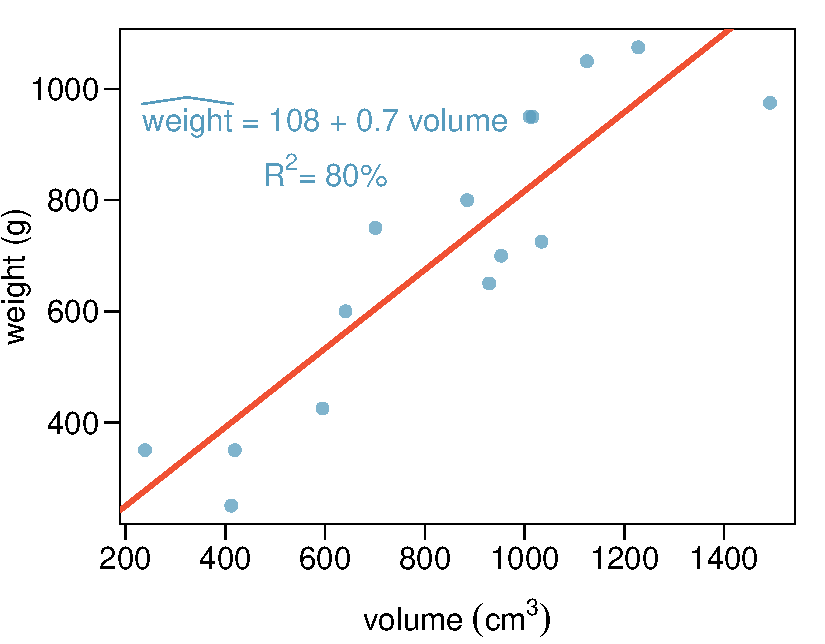
\includegraphics[width=\textwidth]{figures/weight_volume.pdf}
\end{center}
\end{column}
\end{columns}

\end{frame}
%%%%%%%%%%%%%%%%%%%%%%%%%%%%%%%%%%%%%%%%%%%%%%%%%%%%%%%%%%%%%%%%%%%%%%%%
\begin{frame}
\frametitle{But cover type matters}

Coloring the same scatterplot by cover type shows the line is missing something.

\begin{columns}[T]
\begin{column}{0.5\textwidth}
\begin{center}
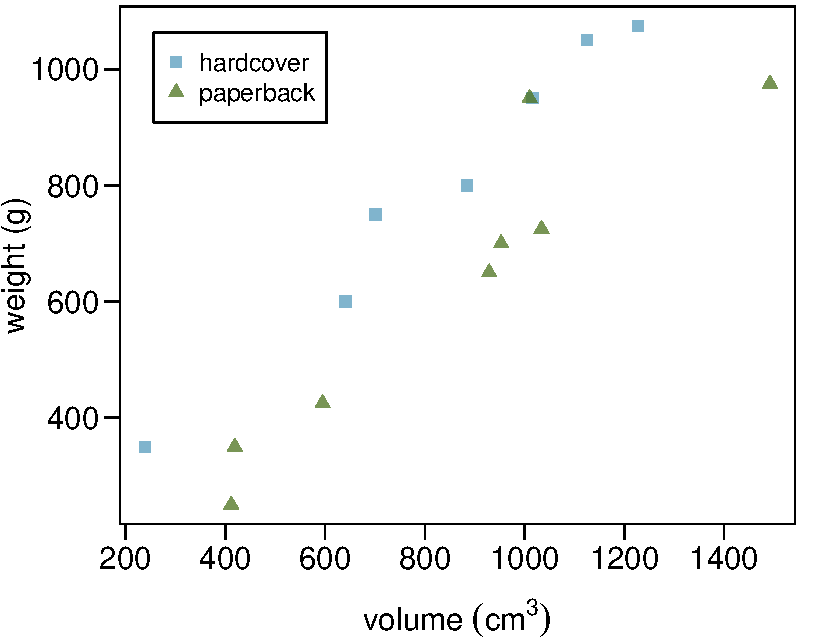
\includegraphics[width=0.92\textwidth]{figures/weight_volume_cover.pdf}
\end{center}
\end{column}
\begin{column}{0.5\textwidth}
\dq{At the same volume, which cover type tends to weigh more?}
\end{column}
\end{columns}

\end{frame}
%%%%%%%%%%%%%%%%%%%%%%%%%%%%%%%%%%%%%%%%%%%%%%%%%%%%%%%%%%%%%%%%%%%%%%%%
\begin{frame}
\frametitle{Model 2: adding cover type}

Define an indicator, with hardcover as the reference level:
$$
\text{cover:pb}=\begin{cases}
1, & \text{paperback book},\\
0, & \text{hardcover book}.
\end{cases}
$$
Fitting \texttt{weight $\sim$ volume + cover} gives:

{\small
\begin{center}
\begin{tabular}{l rrr r}
\toprule
 & Estimate & Std. Error & t value & Pr($>$$|$t$|$) \\
\midrule
(Intercept) & 197.96 & 59.19 & 3.34 & 0.01 \\
volume & 0.72 & 0.06 & 11.67 & 0.00 \\
cover:pb & $-184.05$ & 40.49 & $-4.55$ & 0.00 \\
\bottomrule
\end{tabular}
\end{center}}

\pause
\[ \widehat{\text{weight}} = 197.96 + 0.72\,\text{volume} - 184.05\,\text{cover:pb} \]

\end{frame}
%%%%%%%%%%%%%%%%%%%%%%%%%%%%%%%%%%%%%%%%%%%%%%%%%%%%%%%%%%%%%%%%%%%%%%%%
\begin{frame}
\frametitle{Same model, two lines}

Plug the indicator in and the single model splits into one line per group.

\hl{Hardcover:} plug in $\orange{0}$
\begin{align*}
\widehat{\text{weight}} &= 197.96 + 0.72\,\text{volume} - 184.05\times \orange{0}\\
&= 197.96 + 0.72\,\text{volume}
\end{align*}
\pause
\hl{Paperback:} plug in $\orange{1}$
\begin{align*}
\widehat{\text{weight}} &= 197.96 + 0.72\,\text{volume} - 184.05\times \orange{1}\\
&= 13.91 + 0.72\,\text{volume}
\end{align*}
\end{frame}
%%%%%%%%%%%%%%%%%%%%%%%%%%%%%%%%%%%%%%%%%%%%%%%%%%%%%%%%%%%%%%%%%%%%%%%%
\begin{frame}
\frametitle{Visualizing the model: parallel slopes}

\begin{columns}[T]
\begin{column}{0.55\textwidth}
\begin{center}
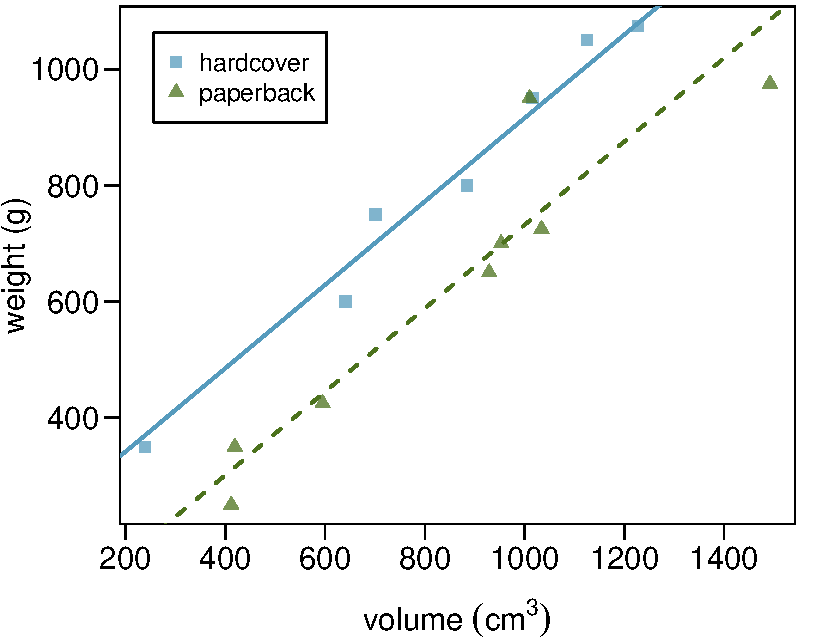
\includegraphics[width=\textwidth]{figures/weight_volume_cover_lines.pdf}
\end{center}
\end{column}
\begin{column}{0.45\textwidth}
\keyidea[-- Parallel slopes]{The indicator shifts the \emph{intercept} but not the \emph{slope}: both lines rise at $0.72$ g per cm$^3$, and the paperback line sits $184$ g lower.}

The vertical gap between the lines is equal to the cover coefficient.
\end{column}
\end{columns}

\end{frame}
%%%%%%%%%%%%%%%%%%%%%%%%%%%%%%%%%%%%%%%%%%%%%%%%%%%%%%%%%%%%%%%%%%%%%%%%
\begin{frame}
\frametitle{Applying the template: the volume coefficient}
\[ \widehat{\text{weight}} = 197.96 + 0.72\,\text{volume} - 184.05\,\text{cover:pb} \]
Run the five steps on $\widehat{\beta}_1=0.72$:

\vspace{-0.3em}
{\footnotesize
\begin{enumerate}
\item Response: \textbf{weight}, in grams.
\pause
\item Predictor: \textbf{volume}, in cm$^3$.
\pause
\item One-unit change: a book $1$ cm$^3$ larger.
\pause
\item Conditional phrase: \hl{holding cover type fixed}.
\pause
\item Direction and units: weight goes \textbf{up} by $0.72$ \textbf{grams}.
\end{enumerate}}

\pause
\vspace{-0.4em}
\workedexample[volume]{Among books with the same cover type, a book $1$ cm$^3$ larger is predicted to weigh about $0.72$ g more.}

\end{frame}
%%%%%%%%%%%%%%%%%%%%%%%%%%%%%%%%%%%%%%%%%%%%%%%%%%%%%%%%%%%%%%%%%%%%%%%%
\begin{frame}
\frametitle{The other two coefficients}
\[ \widehat{\text{weight}} = 197.96 + 0.72\,\text{volume} - 184.05\,\text{cover:pb} \]
\begin{itemize}
\item \hl{Cover ($-184.05$):} the ``one-unit change'' is switching the indicator from $0$ to $1$. Holding volume fixed, a paperback is predicted to weigh about $184$ g \emph{less} than a hardcover.
\pause
\item \hl{Intercept ($197.96$):} set every predictor to $0$ --- a hardcover book of zero volume, predicted to weigh $198$ g.
\end{itemize}

\pause
\caution{The intercept is not meaningful here: no book has zero volume. It only sets the height of the two lines.}

\end{frame}
%%%%%%%%%%%%%%%%%%%%%%%%%%%%%%%%%%%%%%%%%%%%%%%%%%%%%%%%%%%%%%%%%%%%%%%%
\begin{frame}{Activity 2}
\activity[-- interpreting coefficients]{%
\textbf{Worksheet Part 2:} for the fitted book model
\[ \widehat{\text{weight}} = 197.96 + 0.72\,\text{volume} - 184.05\,\text{paperback}, \]
\begin{enumerate}
\item name the response, predictors, and reference level;
\item interpret $0.72$ and $-184.05$ in context, with ``holding fixed'' language;
\item decide whether the intercept is practically meaningful.
\end{enumerate}}
\end{frame}
%%%%%%%%%%%%%%%%%%%%%%%%%%%%%%%%%%%%%%%%%%%%%%%%%%%%%%%%%%%%%%%%%%%%%%%%
\begin{frame}
\frametitle{Prediction}

\pq{Which is the correct calculation for the predicted weight of a \emph{paperback} book with volume $600$ cm$^3$?
\begin{enumerate}
\item $197.96 + 0.72\times 600 - 184.05\times 1$
\item $184.05 + 0.72\times 600 - 197.96\times 1$
\item $197.96 + 0.72\times 600 - 184.05\times 0$
\item $197.96 + 0.72\times 1 - 184.05\times 600$
\end{enumerate}}

\pause
\solnbox{(1). A paperback has $\text{cover:pb}=1$, so
$\widehat{\text{weight}} = 197.96 + 432 - 184.05 = 445.91$ grams.}

\end{frame}
%%%%%%%%%%%%%%%%%%%%%%%%%%%%%%%%%%%%%%%%%%%%%%%%%%%%%%%%%%%%%%%%%%%%%%%%
\begin{frame}{Activity 3}
\activity[-- one model, two lines]{%
\textbf{Worksheet Part 3:} using the same book model,
\begin{enumerate}
\item write the fitted equation for each cover type;
\item predict the weight of a hardcover and of a paperback book with volume $900$ cm$^3$.
\end{enumerate}}
\end{frame}
%%%%%%%%%%%%%%%%%%%%%%%%%%%%%%%%%%%%%%%%%%%%%%%%%%%%%%%%%%%%%%%%%%%%%%%%
\section{$R^2$ and adjusted $R^2$}
%%%%%%%%%%%%%%%%%%%%%%%%%%%%%%%%%%%%%%%%%%%%%%%%%%%%%%%%%%%%%%%%%%%%%%%%
\begin{frame}
\frametitle{$R^2$ with several predictors}

In simple regression we used $R^2=r^2$. With several predictors there is no single correlation between ``$x$'' and $y$, so we fall back on the definition:

\formula{Coefficient of determination}{%
\[ R^2 = \frac{\text{explained variability in }y}{\text{total variability in }y} \]}

We get these two quantities by splitting the total variability in $y$ into a part the model explains and a part it does not (an \hl{analysis of variance}).

\end{frame}
%%%%%%%%%%%%%%%%%%%%%%%%%%%%%%%%%%%%%%%%%%%%%%%%%%%%%%%%%%%%%%%%%%%%%%%%
\begin{frame}
\frametitle{Sum of squares}

The \hl{state poverty data} (Lecture 4): predicting poverty from \% female householder.

{\footnotesize
\begin{center}
\begin{tabular}{lrrrrr}
\toprule
 & Df & Sum Sq & Mean Sq & F value & Pr($>$F) \\
\midrule
female\_house & 1 & 132.57 & 132.57 & 18.68 & 0.00 \\
Residuals & 49 & 347.68 & 7.10 &  &  \\
\midrule
Total & 50 & 480.25 & & & \\
\bottomrule
\end{tabular}
\end{center}}

\pause
\vspace{-0.8em}
{\footnotesize
\begin{align*}
SS_{Total} &= \textstyle\sum(y-\bar{y})^2 = 480.25 &&\orange{\text{total}}\\
SS_{Error} &= \textstyle\sum e_i^2 = 347.68 &&\orange{\text{unexplained}}\\
SS_{Model} &= SS_{Total}-SS_{Error} = 132.57 &&\orange{\text{explained}}
\end{align*}}

\pause
\vspace{-1.0em}
\[ R^2 = \frac{SS_{Model}}{SS_{Total}} = \frac{132.57}{480.25} = 0.28 \]

\end{frame}
%%%%%%%%%%%%%%%%%%%%%%%%%%%%%%%%%%%%%%%%%%%%%%%%%%%%%%%%%%%%%%%%%%%%%%%%
\begin{frame}
\frametitle{Why $R^2$ alone is not enough}

Now add \% white as a second predictor:

{\small
\begin{center}
\begin{tabular}{l c}
\toprule
 & $R^2$ \\
\midrule
Model 1: female\_house & 0.28 \\
Model 2: female\_house + white & 0.29 \\
\bottomrule
\end{tabular}
\end{center}}

$R^2$ went \emph{up}. Does that mean \% white belongs in the model?

\pause
\caution{Adding \emph{any} predictor --- even a useless one --- can only push $R^2$ up. So $R^2$ always favors the bigger model, and on its own it can never tell us whether a predictor earns its place.}

\pause
We need a measure that \hl{charges a price} for each extra predictor.

\end{frame}
%%%%%%%%%%%%%%%%%%%%%%%%%%%%%%%%%%%%%%%%%%%%%%%%%%%%%%%%%%%%%%%%%%%%%%%%
\begin{frame}
\frametitle{Adjusted $R^2$}

\formula{Adjusted $R^2$}{%
\[ R^2_{adj} = 1 - \pr{ \frac{SS_{Error}}{SS_{Total}} \times \frac{n-1}{n-p-1} } \]
where $n$ is the number of cases and $p$ the number of predictors.}

\begin{itemize}
\item The factor $\frac{n-1}{n-p-1}$ is a \hl{penalty} that grows with $p$.
\item $R^2_{adj}$ is always smaller than $R^2$.
\item A predictor only raises $R^2_{adj}$ if it improves the fit \emph{enough to pay for the penalty}.
\item So we prefer models with the higher $R^2_{adj}$.
\end{itemize}

\end{frame}
%%%%%%%%%%%%%%%%%%%%%%%%%%%%%%%%%%%%%%%%%%%%%%%%%%%%%%%%%%%%%%%%%%%%%%%%
\begin{frame}
\frametitle{Calculating adjusted $R^2$}

Model 2 (\% female householder $+$ \% white), with $n=51$ and $p=2$:

{\small
\begin{center}
\begin{tabular}{lrrrrr}
\toprule
 & Df & Sum Sq & Mean Sq & F value & Pr($>$F) \\
\midrule
female\_house & 1 & 132.57 & 132.57 & 18.74 & 0.0001 \\
white & 1 & 8.21 & 8.21 & 1.16 & 0.2868 \\
Residuals & 48 & 339.47 & 7.07 &  &  \\
\midrule
Total & 50 & 480.25 & & & \\
\bottomrule
\end{tabular}
\end{center}}

\pause
\vspace{-0.4em}
{\small
\begin{align*}
R^2_{adj} &= 1 - \pr{ \frac{339.47}{480.25} \times \frac{51-1}{51-2-1} }
= 1 - \pr{ \frac{339.47}{480.25} \times \frac{50}{48} } = 0.26
\end{align*}}

\pause
\vspace{-0.4em}
Model 1 also had $R^2_{adj}=0.26$. So adding \% white pushed $R^2$ up ($0.28\to0.29$) but left $R^2_{adj}$ \emph{unchanged}, so it did not improve predictive performance. 

\end{frame}
%%%%%%%%%%%%%%%%%%%%%%%%%%%%%%%%%%%%%%%%%%%%%%%%%%%%%%%%%%%%%%%%%%%%%%%%
\begin{frame}
\frametitle{What if we just keep adding predictors?}

An experiment, starting from Model 1 (\% female householder, $R^2_{adj}=0.26$):

\begin{itemize}
\item One at a time, add predictors of \emph{pure noise}: random numbers with no connection to poverty.
\item Refit the model after each addition and record $R^2$ and $R^2_{adj}$.
\end{itemize}

\pause
\dq{What will happen to $R^2$? What \emph{should} a good measure of fit do?}
\end{frame}
%%%%%%%%%%%%%%%%%%%%%%%%%%%%%%%%%%%%%%%%%%%%%%%%%%%%%%%%%%%%%%%%%%%%%%%%
\begin{frame}
\frametitle{What if we just keep adding predictors?}

\begin{center}
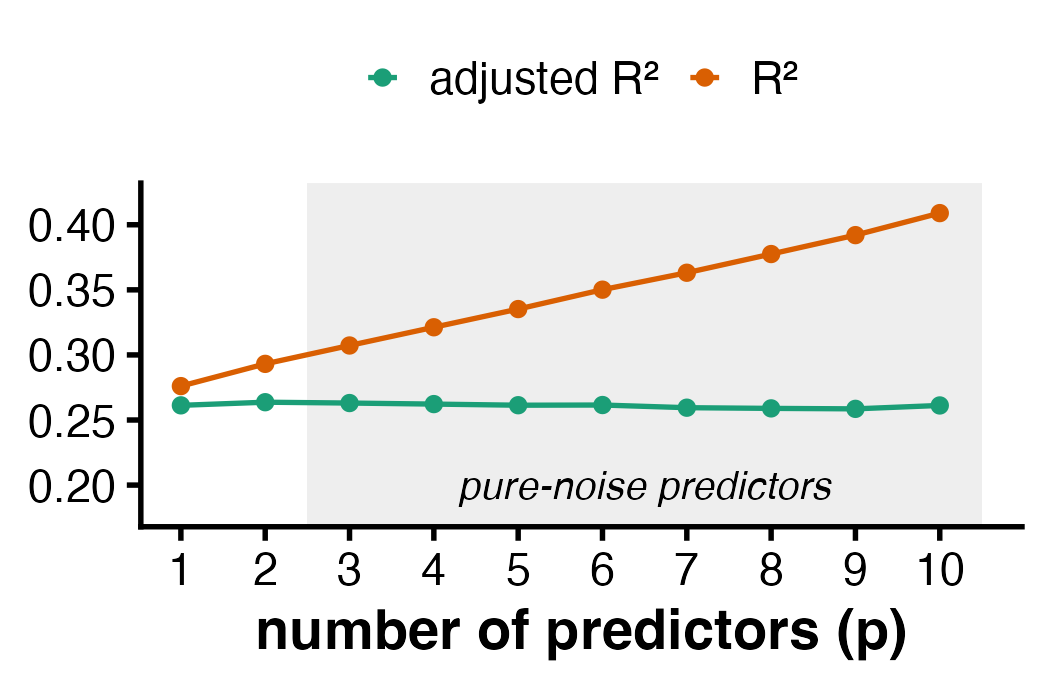
\includegraphics[width=0.6\textwidth]{figures/r2-vs-adjr2.png}
\end{center}

\vspace{-0.4em}
\begin{itemize}
\item $R^2$ climbs to $0.41$ on noise alone: each added predictor lets least squares fit the sample a little better.
\item $R^2_{adj}$ never leaves $\approx0.26$: the penalty absorbs the fake improvement.
\end{itemize}

\end{frame}
%%%%%%%%%%%%%%%%%%%%%%%%%%%%%%%%%%%%%%%%%%%%%%%%%%%%%%%%%%%%%%%%%%%%%%%%
\begin{frame}
\frametitle{Did cover type improve the model?}

\begin{center}
\renewcommand\arraystretch{1.2}
\begin{tabular}{l l c c}
\toprule
Model & Predictors & $R^2$ & Adjusted $R^2$ \\
\midrule
Model 1 & volume & 0.803 & 0.787 \\
Model 2 & volume + cover & 0.927 & 0.915 \\
\bottomrule
\end{tabular}
\end{center}

\pause
Both $R^2$ \emph{and} adjusted $R^2$ jump sharply, so cover type adds real explanatory information.
\end{frame}
%%%%%%%%%%%%%%%%%%%%%%%%%%%%%%%%%%%%%%%%%%%%%%%%%%%%%%%%%%%%%%%%%%%%%%%%
\begin{frame}
\frametitle{Activity 4}

\activity[-- comparing models]{%
\textbf{Worksheet Part 4:} three models predict apartment rent.

{\small
\begin{center}
\begin{tabular}{l l c c}
\toprule
Model & Predictors & $R^2$ & Adj.\ $R^2$ \\
\midrule
A & size & 0.61 & 0.60 \\
B & size + bedrooms & 0.64 & 0.62 \\
C & size + bedrooms + random ID & 0.65 & 0.60 \\
\bottomrule
\end{tabular}
\end{center}}

Which model would you choose, and what does model C tell you about $R^2$?}

\end{frame}
%%%%%%%%%%%%%%%%%%%%%%%%%%%%%%%%%%%%%%%%%%%%%%%%%%%%%%%%%%%%%%%%%%%%%%%%
\begin{frame}{Activity 4}
\solnbox{Model B: highest adjusted $R^2$ with meaningful predictors. Model C has the highest $R^2$ of all, yet its extra predictor is a \emph{random ID code}. That is exactly why $R^2$ alone cannot choose a model.}
\end{frame}
%%%%%%%%%%%%%%%%%%%%%%%%%%%%%%%%%%%%%%%%%%%%%%%%%%%%%%%%%%%%%%%%%%%%%%%%
\section{Wrap-up}
%%%%%%%%%%%%%%%%%%%%%%%%%%%%%%%%%%%%%%%%%%%%%%%%%%%%%%%%%%%%%%%%%%%%%%%%
\begin{frame}
\frametitle{Key takeaways}

\begin{itemize}
\item Read every coefficient \emph{conditionally}: holding the other predictors fixed.
\item A categorical predictor enters through $k-1$ indicators; the omitted level is the reference.
\item A single indicator gives \hl{parallel slopes}: same slope, shifted intercept.
\item Compare models with \hl{adjusted $R^2$}: unlike $R^2$, it penalizes useless predictors.
\end{itemize}

\end{frame}

%%%%%%%%%%%%%%%%%%%%%%%%%%%%%%%%%%%%%%%%%%%%%%%%%%%%%%%%%%%%%%%%%%%%%%%%

%%%%%%%%%%%%%%%%%%%%%%%%%%%%%%%%%%%%
% End document
%%%%%%%%%%%%%%%%%%%%%%%%%%%%%%%%%%%%

\end{document}
